\documentclass[aps,reprint,superscriptaddress,10pt]{revtex4-2}
\usepackage{kotex}
\usepackage[HWP]{dhucs-interword}
\usepackage[dvips]{color}
\usepackage{graphicx}
\usepackage{bm}
\usepackage{amsmath}
\usepackage{tikz}
\usepackage{mhchem}
\usepackage{booktabs}
\usepackage{multirow}
\usepackage{array}
\usepackage{tikz}

\begin{document}
\title{응집물질물리실험 예비보고서 \\
\small 실험주제 : Hall Effect}

\author{HuiJae-Lee}

\affiliation{Physics Department, Inha University}
\email{hjlee6674@inha.edu}

\date{\today}


\begin{abstract}
실험을 통해 홀 효과가 발생하는 원리과 과정을 이해하고 p형, n형 반도체의 홀 저항과 홀 계수를 
측정하여 그 특성과 다른 요소들 사이의 관계를 알아본다.
\end{abstract}
 
 \maketitle
 
\section[Introduction]{Introduction}
전류가 흐르는 도선이 자기장에 수직하게 놓여있으면 로렌츠 법칙에 의해 전류와 자기장에 수직한 방향으로
힘을 받는다. 이는 도선에 내에서 흐르는 전자가 힘을 받는다는 것을 의미한다. 이로인해
전자는 도선의 한쪽 방향에 몰리게 되고 전류가 흐르는 방향에 수직한 방향으로 전압이 발생한다.

\section{Experiment}

\subsection{Theory}

\subsubsection{Hall Effect}
자유전자의 운동량은 파동 벡터 $\vec{k}$와 다음의 관계가 있다.
\begin{align}\label{eq:1-1}
  m\vec{v} = \hbar \vec{k}
\end{align}
전기장 $\vec{E}$와 자기장 $\vec{E}$ 내에서 전하가 $-e$인 전자에 작용하는 힘은 로렌츠 법칙에
의해
\begin{align}\label{eq:1-2}
  \vec{F} = m\frac{d\vec{v}}{dt} = \hbar\frac{d\vec{k}}{dt}
  =-e\left(\vec{E}+\frac{1}{c}\vec{v} \times \vec{B}\right)
\end{align}
가 된다.충돌시간 $\tau$에 대해 $\frac{1}{\tau}$의 비율로 일어나는 충돌에 대한 운동방정식은
\begin{align}\label{eq:1-3}
  \vec{F} = \hbar\left(\frac{d}{dt}+\frac{1}{\tau}\right)\delta\vec{k}
\end{align}
로 쓸 수 있다. $\delta\vec{k}$ 페르미 공의 변위이다. 따라서 식~\eqref{eq:1-1}에 의해
\begin{align}
  m\left(\frac{d}{dt}+\frac{1}{\tau}\right)\vec{v}
  =-e\left(\vec{E}+\frac{1}{c}\vec{v} \times \vec{B}\right)
\end{align}
이다. 이로부터
\begin{align}
  \begin{split}
    m\left(\frac{d}{dt}+\frac{1}{\tau}\right)v_x &= -e\left(E_x+\frac{B}{c}v_y\right), \\
    m\left(\frac{d}{dt}+\frac{1}{\tau}\right)v_y &= -e\left(E_y-\frac{B}{c}v_x\right), \\
    m\left(\frac{d}{dt}+\frac{1}{\tau}\right)v_z &= -eE_z
  \end{split}
\end{align}
임을 알 수 있다. 정적인 전기장에서 위 세 식을 시간에 대해 적분하면
\begin{align}
  \begin{split}\label{eq:1-4}
    v_x &= -\frac{e\tau}{m}E_x-\omega_c \tau v_y,  \\
    v_y &= -\frac{e\tau}{m}E_y+\omega_c \tau v_x,  \\
    v_z &= -\frac{e\tau}{m}E_z
  \end{split}
\end{align}
를 얻는다. $\omega_c=\frac{eB}{mc}$는 사이클로트론 진동수라 부르는 양이다.

\begin{figure}[htbp]
  \centering
  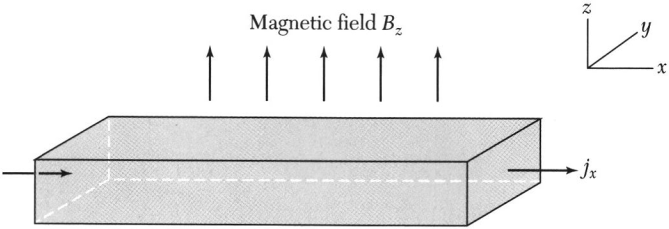
\includegraphics[scale = 0.35]{1-1.png}
  \caption{}
  \label{fig:1-1}
\end{figure}
FIG.~\ref{fig:1-1}과 같이 직사각형 단면을 가진 막대 모양의 시료가 자기장 $B_z$에 놓여있다고
가정하자. 이 시료의 양끝에 가해진 전기장 $E_x$는 시료 막대를 따라 전류 $I_x$를 흐르게 한다.

\begin{figure}[htbp]
  \centering
  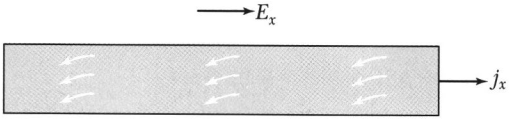
\includegraphics[scale = 0.4]{1-2.png}
  \caption{}
  \label{fig:1-2}
\end{figure}

FIG.~\ref{fig:1-2}와 같이 가로 방향의 전기장 $E_x$와 세로 방향의 자기장 $B_y$ 속에 놓여 있는
막대 모양의 시료에서 전류가 시료에서 $y$쪽 방향으로 흘러나오지 못할 경우 $\delta v_y=0$이어야
한다. 식~\eqref{eq:1-4}으로 부터
\begin{align}
  E_y = -\omega_c \tau E_x = -\frac{eB\tau}{mc}E_x
\end{align}
를 만족해야함을 알 수 있다. 이 때 다음과 같이 정의되는 양 $R_H$를 홀 계수라 부른다.
\begin{align}
  R_H = \frac{E_y}{j_xB}
\end{align}
$j_x = -nev_x=\frac{ne^2\tau}{m}E_x$이므로
\begin{align}
  R_H = -\frac{eB\tau E_x/mc}{ne^2\tau E_xB/m}=-\frac{1}{nec}
\end{align}
로 쓸 수 있다.

% 자기장 $\vec{B}$를 가로지르는 방향으로 전류 $\vec{I}$가 흐를 때 $\vec{I} \times \vec{B}$
% 방향으로 전기장이 생성된다.


\subsection{Experimental Methods}
\begin{itemize}
  \item[1 .] 가우스미터를 전자석 사이 중앙에 잘 위치시킨다.
  가우스미터를 통해 전자석의 자기장 크기를 전류의 값으로 치환한다.
  \item[2 .] 전자석의 자기장 세기를 6000 G까지 100 G씩 올려가며 가우스미터의 
  전류 값을 기록한다.
  \item[3 .] n형 반도체 샘플을 홀 전압 측정 장치에 연결하고 측정 장치의
  off set을 0으로 설정한다. 이 때 샘플이 전자석의 중앙에 위치하도록 잘 조정해준다. 
  \item[4 .] 샘플에 흐르는 전류를 측정할 값(2 mA, 4 mA, 6 mA)에 맞춘 후, 자기장을
  올려가며 홀 전압을 측정한다.
  \item[5 .] 샘플을 p형 반도체로 교체하여 과정 3, 4를 반복한다.
\end{itemize}

\nocite{*} 
\bibliography{ref}



%\begin{thebibliography}{9}
%\end{thebibliography}

\vfill
\end{document}